%!TEX root = ../main.tex
%%%%%%%%%%%%%%%%%%%%%%%%%%%%%%%%%%
% Links:
%
% Difficulty:
% Companies: 
%%%%%%%%%%%%%%%%%%%%%%%%%%%%%%%%%%


\chapter{Least Recently Used Cache}
\label{ch:LRU_cache}
\section*{Introduction}
Caches are piece of hardwoare of software systems responsible to store data that allow the system to respond to future requests faster. Usually such data is the result of earlier computation 
of it could data that was copied over from somewhere else  (following the principle of temporal and spatial locality which states that applications are more likely to access data that has been accessed recently and/or that sit close in memory).  
Caches are essential piece of nowadays computer systems and we find them at every level: from CPUs and HDDs (see Figure \ref{fig:LRU_cache:cpu_cache}) that have dedicated expensive blocks of memory that for temporary storage of data that is likely to be used again, to 
browsers or webserver (see Figure \ref{fig:LRU_cache:web_cache}) that use caches to try and lower the latency of your browsing.


Clearly caches have finite size and eventually they get full and therefore we run into the issue of deciding what to delete from it in order to make some space available for the new data. There are many policies that can be employed here like for example:
\begin{itemize}
	\item LRU: discards the least recently used items first;
	\item FIFO: evice the oldest data first (regardless of whether it has been accessed recently);
	\item RR: (random replacement) that, as the name suggests, removes one or more random cache entries.
\end{itemize}

The problem we will solve in this chapter is about implementing a LRU cache so that all of its supported operation are carried out with the best time efficiency possible. As we will see, solving this problem by making all operations $log(n)$ is actually pretty easy, but 


\begin{figure}
	\centering
	\begin{subfigure}[t]{0.49\textwidth}
		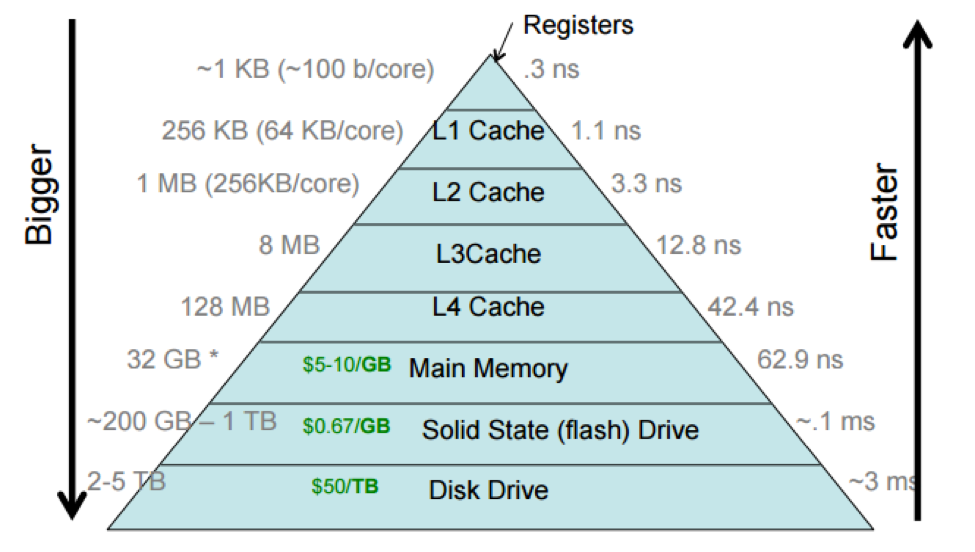
\includegraphics[width=1\linewidth]{sources/LRU_cache/images/cpu_caches}
		\caption{Caches (notice that there are multiple level of it) are at the top of the memory hierarchy of modern computers. See Table \ref{tab:refernce_latencies} for a more detailed account of the latencies figures for each and every memory level of the hierarchy. The figures on size and latency showed are for a typical desktop computer. Use \inline{getconf -a | grep CACHE} or \inline{lscpu} to check the actual cache size in your system.}
		\label{fig:LRU_cache:cpu_cache}
	 \end{subfigure}
	\hfill
	\begin{subfigure}[t]{0.49\textwidth}
		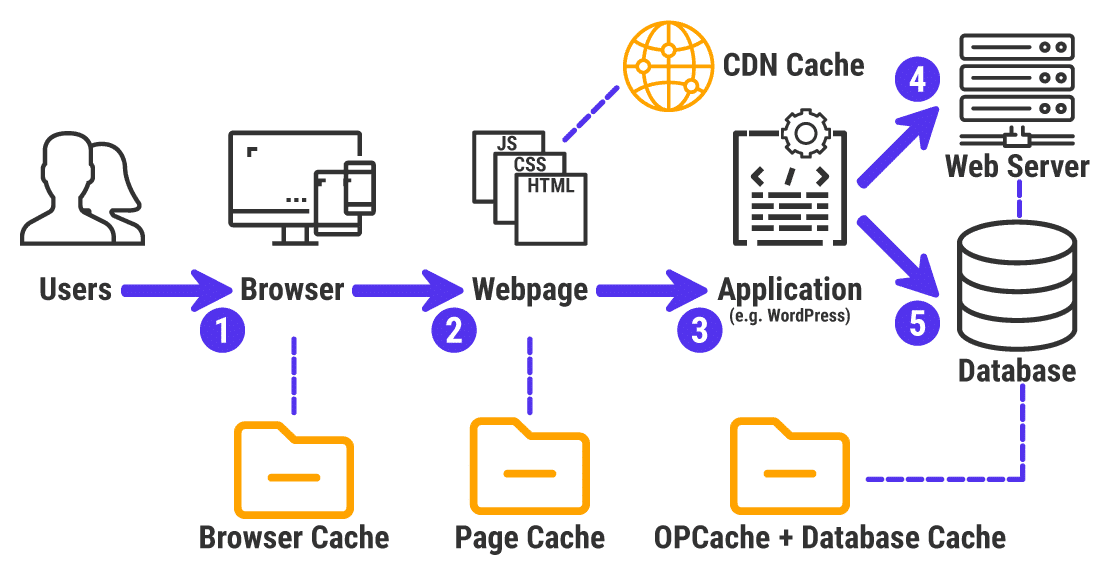
\includegraphics[width=1\linewidth]{sources/LRU_cache/images/web_caches}
		\caption{Caches in the internet. We can see caches being used at every level. Even the database might cache recently used data in memory.}
		\label{fig:LRU_cache:web_cache}
	 \end{subfigure}
	 \caption[]{dsjfhgdkj}
	  \label{fig:LRU_cache:caches_example}
\end{figure}


\section{Problem statement}
\begin{exercise}
\label{example:LRU_cache:exercice1}
Implement the two two public methods of the \inline{LRUCache} interface below. The class should behave like a LRU cache of capacity \inline{n} that is given as a parameter.
\begin{itemize}
	\item \inline{std::optional<Value> get(Key k)} retuns the value associated with the key \inline{k}. If \inline{k} is not in the cache, the function returns \inline{std::nullptop}. 
	\item \inline{void put(Key k, Value v)} adds or update (depending on whether $k$ is already present in the cache or not) the pair $(k,v)$. If the cache if full i.e. has size $n$ the function evices the least recently used items before inserting $(k,v)$.
\end{itemize}

	%example1
	\begin{example}
		\label{example:LRU_cache:example1}
		\hfill \\ 
		For instance, given a cache \inline{C} of size $2$ (with char keys and int values) then Table \ref{tab:LRU_cache:example1} shows the content after performing an operation on it:

		
	\end{example}


\end{exercise}

% Please add the following required packages to your document preamble:
% \usepackage{graphicx}
\begin{table}[]
	\centering
	\resizebox{\textwidth}{!}{%
	\begin{tabular}{lllr}
		\hline
		\rowcolor[HTML]{C0C0C0} 
		\multicolumn{1}{c}{\cellcolor[HTML]{C0C0C0}\textbf{Operation}} & \multicolumn{1}{c}{\cellcolor[HTML]{C0C0C0}\textbf{Cache}} & \multicolumn{1}{c}{\cellcolor[HTML]{C0C0C0}\textbf{Return}} & \textbf{Comment} \\ \hline
	\inline{get('a')}                       & \inline{\{\}}     & \inline{std::nullopt} & \inline{'a'} $\notin C$ \\
	\inline{put('a',1)}                       & \inline{\{a=1\}}     & - & Put OK \\
	\inline{put('b',2)}                       & \inline{\{a=1\},\{b=2\}}     & - & Put OK \\
	\inline{get('a')}                       & \inline{\{a=1\},\{b=2\}}     & \inline{1} & \inline{'b'} is LRU element now \\
	\inline{get('b')}                       & \inline{\{a=1\},\{b=2\}}     & \inline{2} & \inline{'a'} is LRU element now\\
	\inline{put('c',3)}                       & \inline{\{a=1\},\{c=3\}}     & - & Put OK. \inline{'a'} evicted\\
	\inline{get('a')}                       & \inline{\{a=1\},\{c=3\}}     & \inline{std::nullopt} & \inline{'a'} $\notin C$ anymore\\
	\inline{get('b')}                       & \inline{\{a=1\},\{c=3\}}     & \inline{2} & Get OK\\
	\inline{get('c')}                       & \inline{\{a=1\},\{c=3\}}     & \inline{3} & Get OK

	\end{tabular}%
	}
	\caption{Example of behavior of the a LRU cache.}
	\label{tab:LRU_cache:example1}
	\end{table}

\section{Clarification Questions}

\begin{QandA}
	\item 
	\begin{answered}
		\textit{}
	\end{answered}
	
\end{QandA}

\section{Discussion}
\label{LRU_cache:sec:discussion}


\subsection{Brute-force}
\label{LRU_cache:sec:bruteforce}

\begin{minipage}{\linewidth}
	\lstinputlisting[language=c++, caption={Sample Caption},label=list:LRU_cache]{sources/LRU_cache/LRU_cache_solution1.cpp}
\end{minipage}

